\documentclass[hyperref={pdfpagelabel=false},8pt, handout=show,show notes]{beamer}

\usepackage[utf8x]{inputenc}
\usepackage[T1]{fontenc} 
\usepackage{default}
\usetheme[width=2cm]{Goettingen}
\usepackage{amsmath} 
\usecolortheme{rose}
\usepackage{enumerate}
\usepackage{graphicx}
\usepackage{amsmath} 
\usepackage{lmodern}
\usepackage{subfigure}
\usepackage{float}
\usepackage{wrapfig} 
\usepackage[french]{babel}
\author[]{Alexandre Lacaste, Simon Carrignon\\ 
 Laboratoire des Usages en Technologies d' Information Numérique
}

\usepackage[small]{caption}
\useoutertheme{infolines}
\usepackage{subfigure}
\usepackage[footheight=1em]{beamerthemeboxes}
\usepackage{algorithmicx}
\usepackage{algpseudocode}
\title{Agent Based Pedestrian Model}
\usepackage{algorithm}

\usepackage[]{natbib}
\bibpunct{[}{]}{,}{a}{,}{,}
\begin{document}

\begin{frame}
 \maketitle
\end{frame}

\begin{frame}
 \begin{beamerboxesrounded}{Objectif}
  Mod\'elisation Comportements Pi\'etons.
  \begin{itemize}
   \item Agent Based Model
   \item Ajustement et validation avec donn\'ees r\'eelles 
   \item Comparaison entre mod\`eles
   \item Impactes des modifications de l'environnement
 \end{itemize}


 \end{beamerboxesrounded}
 
\end{frame}

\begin{frame}{Interface netlogo}
\begin{columns}
\begin{column}{.45\textwidth}
Netlogo :
\begin{itemize}
 \item Visualisation rapide
 \item Utilisation bmp pour background
 \item Ajustement simple et rapide des param\`etres
 \item Multi-agent, Agent centr\'e...i
 \item mod\`ele ACACIA (Quera V, Zibetti, etc..)
\end{itemize}

\end{column}

\begin{column}{.5\textwidth}
\begin{figure}
 \centering
 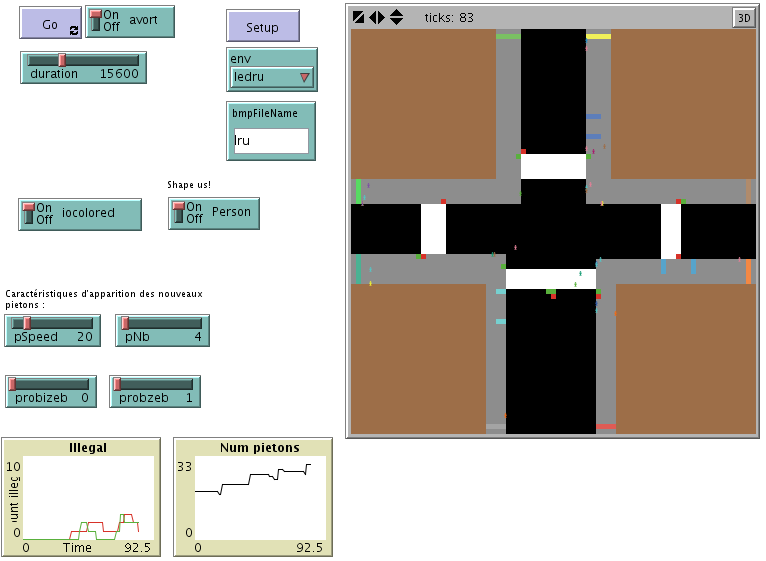
\includegraphics[width=\textwidth]{images/netlogo-printscreen}
\end{figure}
\end{column}

\end{columns}
 
\end{frame}

\begin{frame}{Le mod\`ele na\"if} 


\begin{algorithmic}
\Function{AgentBehavior}{ }
    \Loop
    \If{$FedUp()$} 
    \State $ChooseNewGoal()$
    \EndIf
    \State $FaceGoal()$
    \State $LookAhead()$
    \While{$getProba(patchAhead) < 1$}
    \State $AvoidPatchAhead()$
    \State $LookAhead()$
    \EndWhile
    \State $GoAhead()$ 
    \EndLoop
\EndFunction

\end{algorithmic}

 \end{frame}

\begin{frame}{Premiers resultats}

\begin{figure}
 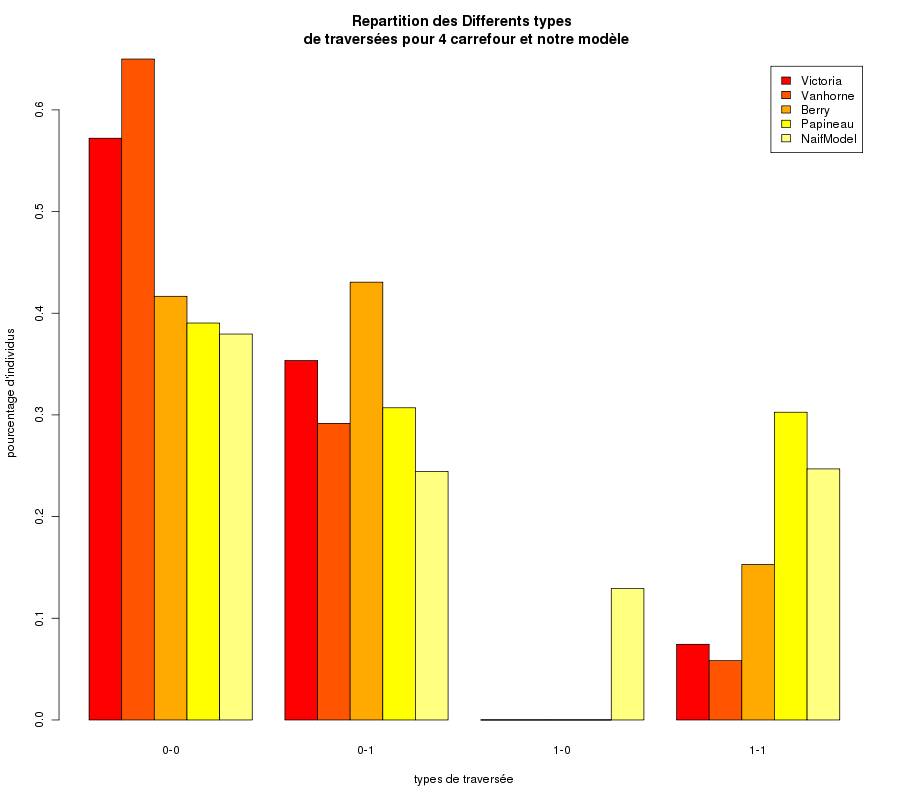
\includegraphics[height=.60\textwidth]{images/BarplotMontrealMode}
\end{figure}
\begin{itemize}
 \item Mod\`ele sur Ledru-Rollin
 \item Similaire \`a Papineau?
 \item Tests de comparaison \`a d\'efinir...
 \item et si similarit\'e ``\'etablie'':
 \begin{itemize}
  \item Que souligne-t-elle?
  \item Comment l'exploiter?
  \item Quels crit\`eres de validation,
  \item affiner les comparaison (ici tr\`es g\'en\'eral : \% global peu significatif)
 \end{itemize}

\end{itemize}



\end{frame}

 
\end{document}
